\section{Spark::Sp\-Stream\-Feedback Class Reference}
\label{classSpark_1_1SpStreamFeedback}\index{Spark::SpStreamFeedback@{Spark::SpStreamFeedback}}
{\tt \#include $<$Sp\-Stream\-Feedback.h$>$}

Inheritance diagram for Spark::Sp\-Stream\-Feedback:\begin{figure}[H]
\begin{center}
\leavevmode
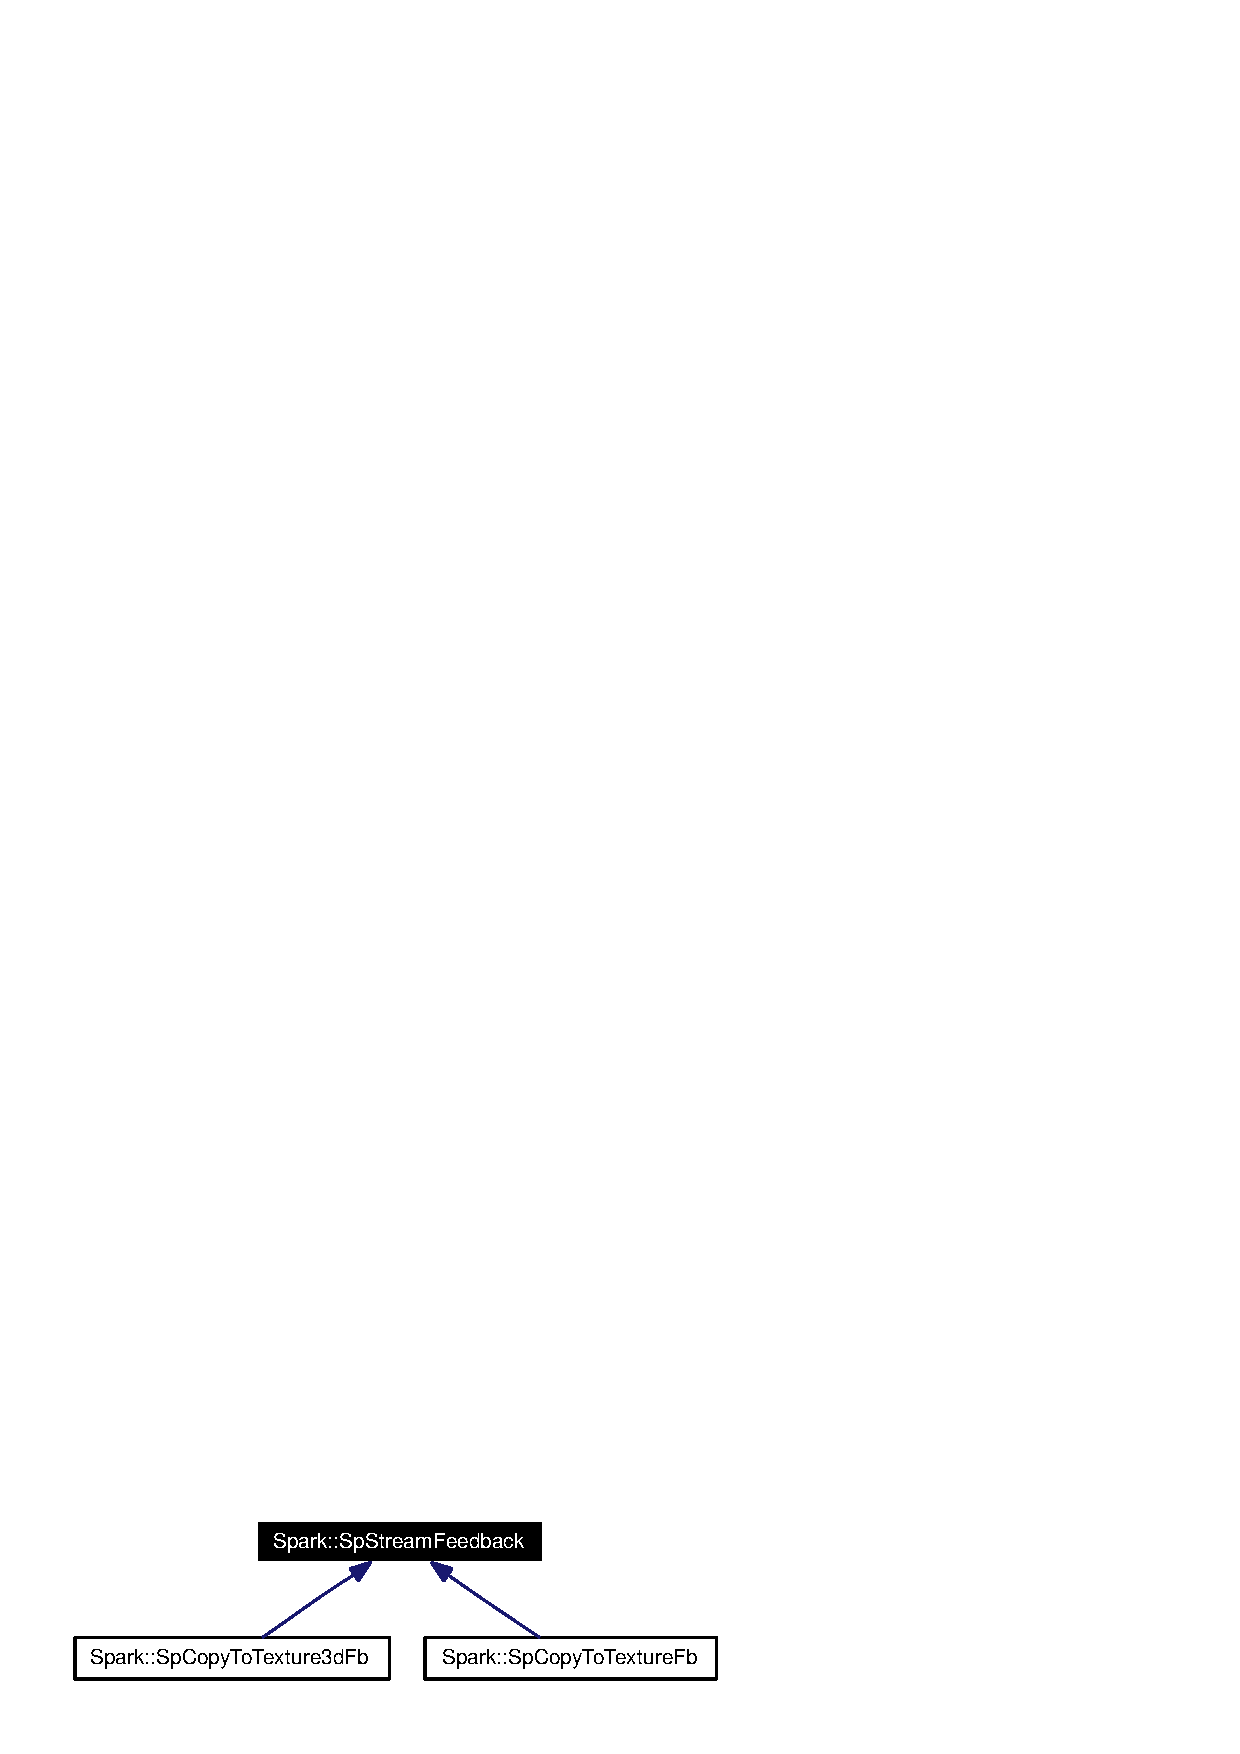
\includegraphics[width=172pt]{classSpark_1_1SpStreamFeedback__inherit__graph}
\end{center}
\end{figure}


\subsection{Detailed Description}
Abstract base class for a stream feedback mechanism for returning results. 

Definition at line 30 of file Sp\-Stream\-Feedback.h.\subsection*{Public Member Functions}
\begin{CompactItemize}
\item 
virtual void {\bf set\-Output\-Texture} (unsigned int ui\-Texture\-Id, int, int, int)=0
\item 
virtual void {\bf update\-Output} ()=0
\end{CompactItemize}


\subsection{Member Function Documentation}
\index{Spark::SpStreamFeedback@{Spark::Sp\-Stream\-Feedback}!setOutputTexture@{setOutputTexture}}
\index{setOutputTexture@{setOutputTexture}!Spark::SpStreamFeedback@{Spark::Sp\-Stream\-Feedback}}
\subsubsection{\setlength{\rightskip}{0pt plus 5cm}virtual void Spark::Sp\-Stream\-Feedback::set\-Output\-Texture (unsigned int {\em ui\-Texture\-Id}, int, int, int)\hspace{0.3cm}{\tt  [pure virtual]}}\label{classSpark_1_1SpStreamFeedback_a0}




Implemented in {\bf Spark::Sp\-Copy\-To\-Texture3d\-Fb} {\rm (p.\,\pageref{classSpark_1_1SpCopyToTexture3dFb_a2})}, and {\bf Spark::Sp\-Copy\-To\-Texture\-Fb} {\rm (p.\,\pageref{classSpark_1_1SpCopyToTextureFb_a2})}.



Referenced by Spark::Sp\-Turbulence\-Op::enable\-Output\-Stream().\index{Spark::SpStreamFeedback@{Spark::Sp\-Stream\-Feedback}!updateOutput@{updateOutput}}
\index{updateOutput@{updateOutput}!Spark::SpStreamFeedback@{Spark::Sp\-Stream\-Feedback}}
\subsubsection{\setlength{\rightskip}{0pt plus 5cm}virtual void Spark::Sp\-Stream\-Feedback::update\-Output ()\hspace{0.3cm}{\tt  [pure virtual]}}\label{classSpark_1_1SpStreamFeedback_a1}




Implemented in {\bf Spark::Sp\-Copy\-To\-Texture3d\-Fb} {\rm (p.\,\pageref{classSpark_1_1SpCopyToTexture3dFb_a3})}, and {\bf Spark::Sp\-Copy\-To\-Texture\-Fb} {\rm (p.\,\pageref{classSpark_1_1SpCopyToTextureFb_a3})}.



The documentation for this class was generated from the following file:\begin{CompactItemize}
\item 
{\bf Sp\-Stream\-Feedback.h}\end{CompactItemize}
